\section{Results and Discussion}
\label{sec:fn_opt:results}

    This section elucidates the optimization outcomes for 20 classical functions, analyzed using three distinct selection 
    strategies: Random, Tournament, and Roulette. The following tables and figures provide an in-depth view of the time 
    efficiency and effectiveness of each phase in the evolutionary process, along with the resultant optimization 
    performance.

    \begin{figure}[ht!]
        \centering
        \begin{subfigure}{.45\textwidth}
            \centering  
            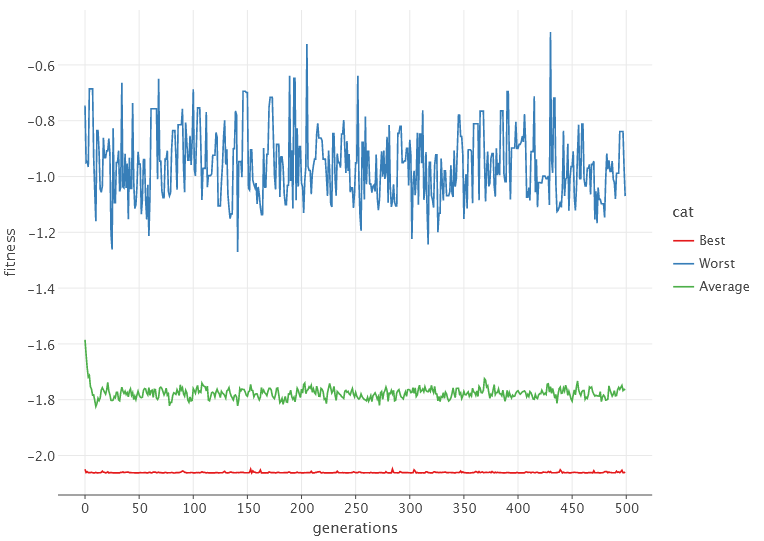
\includegraphics[width=\linewidth]{img/cross_in_tray_random.png}
            \caption{Random Selector}
        \end{subfigure}
        \begin{subfigure}{.45\textwidth}
            \centering
            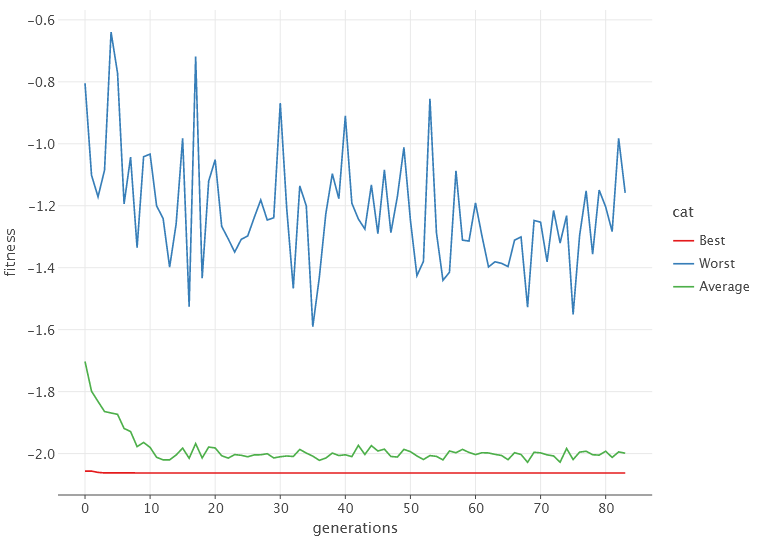
\includegraphics[width=\linewidth]{img/cross_in_tray_tournament.png}
            \caption{Tournament Selector}
        \end{subfigure}
        \begin{subfigure}{.45\textwidth}
            \centering
            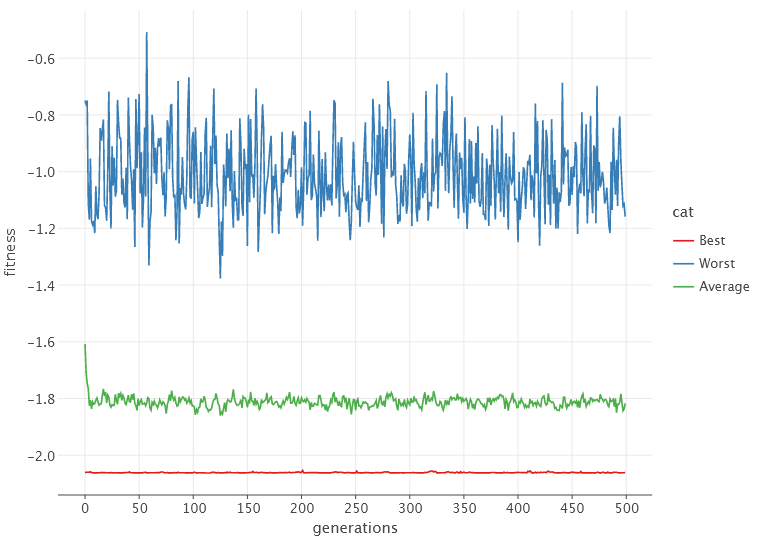
\includegraphics[width=\linewidth]{img/cross_in_tray_roulette.png}
            \caption{Roulette Selector}
        \end{subfigure}
        \caption{Fitness evolution for the Cross-in-tray function under different selection strategies.}
        \label{fig:fn_opt:results:cross_in_tray}
    \end{figure}

    The comparative analysis of the selectors, as depicted in \vref{fig:fn_opt:results:cross_in_tray}, highlights the 
    superior performance of the Tournament Selector over the Random and Roulette Selectors. Notably, the Random and 
    Roulette selectors exhibit comparable outcomes, which can be attributed to the inherent nature of the Roulette 
    Selector. This selector functions as a probabilistic version of the Random Selector, where the selection probability 
    is guided by individual fitness weights. As the evolutionary process progresses, the variance in these weights 
    diminishes, leading to Roulette Selector's behavior increasingly resembling that of the Random Selector.

    It is crucial to observe that while both Random and Roulette selectors occasionally approach or even achieve the
    global optimum, their inherent randomness impedes consistent maintenance of the optimum solution. Conversely, the 
    Tournament Selector, with its more deterministic and competitive selection mechanism, not only reaches but also 
    reliably sustains the optimal solutions once discovered. From this we can conclude that a stagnation termination
    criterion is not suitable for the Random and Roulette selectors, as they are not able to maintain the optimal 
    solution for a long enough period of time, instead a target fitness criterion may be more appropriate.

    Now we will present the results of the optimization process for each selector for each function.
    Each experiment was run 4 times, dropping the first iteration to avoid JVM warmup effects. The results presented are
    the average of the remaining 3 iterations.

    \newpage
    \begin{center}

        \subsection{Random Selector}
            \subimport{results/}{Random.tex}
        \subsection{Tournament Selector}
            \subimport{results/}{Tournament.tex}
        \subsection{Roulette Selector}
            \subimport{results/}{Roulette.tex}
    \end{center}